\documentclass[10pt,a4paper]{article}
% ========================== DO NOT MODIFY =================================== %
\usepackage[a4paper,left=2.0cm,top=2.0cm,right=2.0cm,bottom=2.0cm]{geometry} 
\usepackage{amsmath, mathtools} % If amsmath is required
\usepackage{url}
%\usepackage{times}
\usepackage{newtxtext,newtxmath}    %% use fitting times fonts also in formulas
\usepackage{graphicx}
\usepackage{titling}
\usepackage{authblk}
\usepackage{multicol}
\usepackage{float}
\usepackage{enumitem}
\usepackage[small,compact]{titlesec}
\usepackage[numbers,sort&compress]{natbib}
%\usepackage[T1]{fontenc}
\usepackage[UKenglish]{babel}
\usepackage[small,bf,tableposition=top,figureposition=bottom,skip=2pt]{caption}
\usepackage{subfig}
\usepackage{cleveref}

\graphicspath{{../img/}}

% limit space between floats and text
\setlength{\textfloatsep}{10pt plus 1.0pt minus 2.0pt}
% shrink the list environments
\setlist{noitemsep}
\setlist{nolistsep}

% Shrink the bibliography
  \let\oldthebibliography=\thebibliography
  \let\endoldthebibliography=\endthebibliography
  \renewenvironment{thebibliography}[1]{%
    \begin{oldthebibliography}{#1}%
      \setlength{\parskip}{0ex}%
      \setlength{\itemsep}{0ex}%
  }%
  {%
    \end{oldthebibliography}%
  }

% Format of the front matter
\renewcommand{\Affilfont}{\small}
\setlength{\affilsep}{1ex}
\renewcommand\Authands{, }
\setlength{\droptitle}{-1.634cm}
% ============================================================================ %


% To be able to type european characters without escape sequences
% uncomment according to your operating system, if desired:
% ---------------------------------------------------------------------------- %
% \usepackage[latin1]{inputenc}   %% (Windows, old Linux)
% \usepackage[utf8]{inputenc}     %% (Linux)
% \usepackage[applemac]{inputenc} %% (Mac OS)
% ---------------------------------------------------------------------------- %


%------------------------------- FRONT MATTER -------------------------------- %
\title{3D EIT image reconstruction with GREIT%
\vspace{-2ex}} %remove vertical space
\author[1]{Bart\l{}omiej Grychtol}
\author[2]{Beat M\"uller}
\author[3]{Andy Adler}
\affil[1]{Fraunhofer Project Group for Automation in Medicine and 
Biotechnology, Mannheim, Germany \protect\url{b.grychtol@ipa.fraunhofer.de}}
\affil[2]{Swisstom AG, Landquart, Switzerland}
\affil[3]{Systems and Computer Engineering, Carleton University, Ottawa, Canada}
\date{}
%----------------------------------------------------------------------------- %

\newcommand{\vB}{\mbox{$\mathbf{v}$}}
\newcommand{\xB}{\mbox{$\mathbf{x}$}}
\newcommand{\rB}{\mbox{$\mathbf{r}$}}
\newcommand{\xH}{\mbox{$\mathbf{\hat x}$}}
\newcommand{\xT}{\mbox{$\mathbf{\tilde x}$}}
\newcommand{\XT}{\mbox{$\mathbf{\tilde X}$}}
\newcommand{\nB}{\mbox{$\mathbf{n}$}}
\newcommand{\yB}{\mbox{$\mathbf{y}$}}
\newcommand{\wB}{\mbox{$\mathbf{w}$}}
\newcommand{\AB}{\mbox{$\mathbf{A}$}}
\newcommand{\BB}{\mbox{$\mathbf{B}$}}
\newcommand{\RB}{\mbox{$\mathbf{R}$}}
\newcommand{\IB}{\mbox{$\mathbf{I}$}}
\newcommand{\JB}{\mbox{$\mathbf{J}$}}
%\renewcommand{\PB}{\mbox{$\mathbf{P}$}}
\newcommand{\VB}{\mbox{$\mathbf{V}$}}
\newcommand{\WB}{\mbox{$\mathbf{W}$}}
\newcommand{\XB}{\mbox{$\mathbf{X}$}}
\newcommand{\YB}{\mbox{$\mathbf{Y}$}}
\newcommand{\SG}{\mbox{$\boldsymbol{\Sigma}$}}

 
\begin{document}
\newcommand{\argmin}{\operatornamewithlimits{arg\,min}}
\DeclarePairedDelimiter\norm{\lVert}{\rVert}%
%  \setlength{\abovedisplayskip}{0.5\baselineskip}%
%  \setlength{\belowdisplayskip}{0.5\baselineskip}%
\maketitle
\vspace{-1.5cm}
\thispagestyle{empty}

\begin{multicols}{2}

\noindent {\bf Abstract:} The Graz consensus reconstruction algorithm for EIT 
(GREIT) has become popular in lung EIT. One shortcoming of the original 
formulation of GREIT is its restriction to 2D image reconstruction and so 
planar electrode arrangement. We present an extension of the GREIT algorithm to 
3D and discuss some of the issues that arise.

\section{Introduction}
Since its publication in 2009, the Graz consensus reconstruction algorithm for 
EIT (GREIT) \cite{Adler2009b} has become popular in lung EIT. The original 
formulation and implementation available in EIDORS (\url{www.eidors.org}) was 
limited to cylindrical geometries with planar electrode arrangement. Subsequent 
adaptations allowed reconstructions on arbitrary geometry \cite{Grychtol2011}. 
Recently, Ahn~et~al.~\cite{Ahn2014a} proposed and tested in a 
360-electrode micro-EIT setup an extension of the GREIT algorithm to 3D.
We describe a similar implementation contributed to EIDORS and 
investigate the algorithm's properties. We use a commercially available 
32-electrode EIT system intended for lung imaging.


\section{Methods} 
GREIT is a linear reconstruction for difference EIT. Images are obtained by 
multiplying difference voltage data by a reconstruction matrix \RB\ calculated 
from $k$ (simulated) measurements \yB\ of point target contrasts and the 
corresponding `desired images' \xT\ as
%\begin{equation}
%	\RB = \XT\YB\left(\JB\SG_\mathrm{x}\JB^\intercal + 
%	\lambda\SG_\mathrm{n}\right)^{-1},
%\end{equation}
%where \JB\ is the Jacobian (sensitivity) matrix, $\SG_\mathrm{x}$ and 
%$\SG_\mathrm{n}$ are the image and noise covariances, and $\lambda$ is the 
%hyperparameter. \YB\ and \XT\ are obtained by horizontal concatenation of 
%measurement and image vectors, respectively.
\begin{equation}
\RB = \argmin_{\footnotesize\RB}\sum_k \norm*{\xT^{(k)} - 
\RB\yB^{(k)}}^2_{\wB^{(k)}}
\end{equation}
where $\wB^{(k)}$ is a vector weighting individual desired image elements and 
is commonly set to a scalar value identical for all desired images 
\citep[eq. 13]{Adler2009b}.


One key parameter influencing the properties of the GREIT reconstruction matrix 
is the definition of the desired images. In the original formulation, they are 
circles centered at the point targets' position, with an inner circular zone 
where the amplitude is flat and a zone outside a larger circular boundary where 
the amplitude is zero. Between the two circles, the amplitude 
is supposed to ``gradually decrease''  \cite{Adler2009b}.
We propose to formalize the 
desired image definition by means of a sigmoid function of position
\begin{equation}
f(\rB) = \left(1 + e^{s\left(\left|\rB-\rB_0\right| - R\right)}\right)^{-1},
\end{equation}
where \rB\ is the position vector in 2- or 3D, $\rB_0$ is the target 
center, $R$ is the desired radius and $s$ is a scalar controlling the blur  
(\cref{fig:sigmoid_plot}). $f(\rB)$ can be discretized on pixels or voxels. 

\begin{figure}[H]
\subfloat[$R = 0.5$]%
{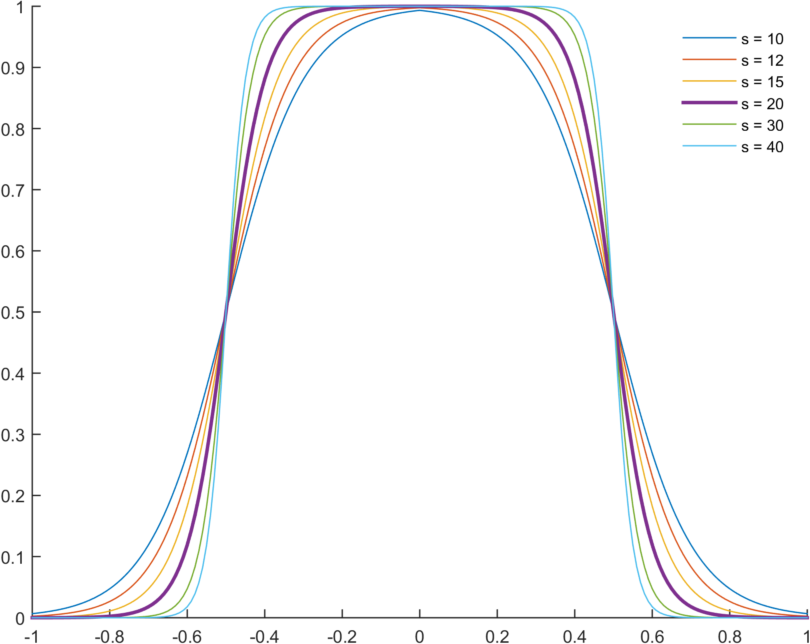
\includegraphics[width=.4\columnwidth]{sigmoid_01a.png}}
\hfill
\subfloat[$R = 0.25$]%
{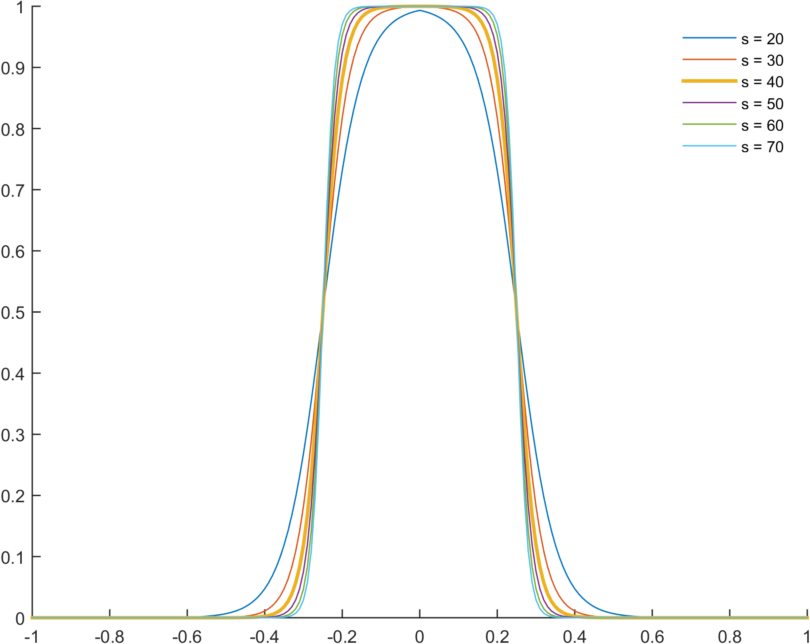
\includegraphics[width=.4\columnwidth]{sigmoid_01b.png}}
\caption{\label{fig:sigmoid_plot}
	Plots of the function $f(x) = 1 / (1 + e^{s(|x|-R)})$ for different values 
	of $s$ with the default value indicated in bold.
	}
\end{figure}
\begin{figure}[H]
\vspace{-5mm}
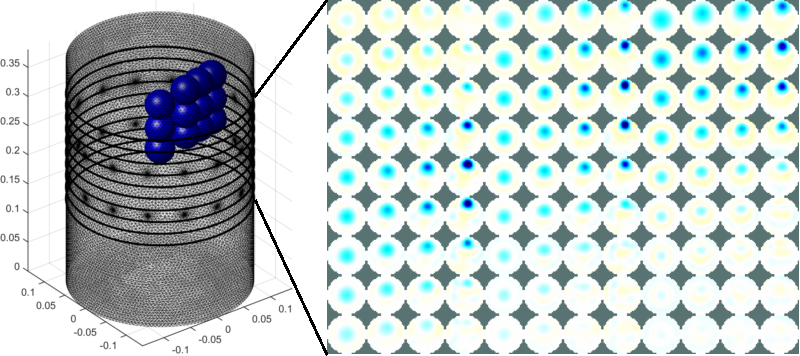
\includegraphics[width=\columnwidth]{tank_recon.pdf}
\caption{\label{fig:tank_recon} \emph{Left:} FE model of a water tank showing 
cut planes between voxel layers and positions of a non-conductive spherical 
target. \emph{Right:} images reconstructed using the proposed algorithm. Each 
row corresponds to one voxel layer, and each column to a different target 
position.}
\end{figure}

\section{Discussion}
Sample 3D reconstruction of data collected with the Pioneer Set (Swisstom AG) 
from a water tank with two layers of 16 electrodes are shown in 
\cref{fig:tank_recon}. Variations in vertical and radial position of a 
non-conductive spherical target are successfully reconstructed. 
As expected, amplitude response and 
resolution fall toward the long axis of the tank and away from the electrode 
plane. On the other hand, ringing seems to be stronger in the electrode planes.

Extension of the GREIT framework to 3D expands the application of this popular 
lung EIT algorithm to other domains, such as head or breast imaging. It also  
rises interesting questions: What is 
the desired image for an out-of-plane target? How, if 
at all, should the desired image amplitude be affected by the measurement 
sensitivity? Is noise figure a suitable way to choose the hyperparameter? How 
many targets are necessary, and how should they be distributed? Are the answers 
dependent on the stimulation pattern?
As experience with 3D imaging in the EIT community grows,
we antipate that solutions will be developed for these issues.

\footnotesize
\bibliographystyle{compact}
\bibliography{library}
% We encourage the use of bibtex, but you can also type the reference 
% the traditional way
%\begin{thebibliography}{}
%\bibitem[1]{Waspaa1} Lyon RF, Mead, C, IEEE 
%Trans. ASSP  36: 1119--1134, 1988.
%\bibitem[2]{Waspaa2} Lee, KF, Automatic Speech Recognition: The Development 
%of the SPHINX SYSTEM, Kluwer Academic Publishers, Boston, 1989.
%\end{thebibliography}
\end{multicols}

\end{document}
